\chapter{Конструкторская часть}

В данной части будут разработаны функциональные схемы разрабатываемого ПО, а также разработаны структуры и алгоритмы, которые будут использованы в ПО.

\section{Функциональные схемы} 

На рисунках \ref{fig:A0} -- \ref{fig:A3} представлено формальное описании разрабатываемого ПО в виде idef0-диаграммы.

\begin{figure}[H]
	\centering
	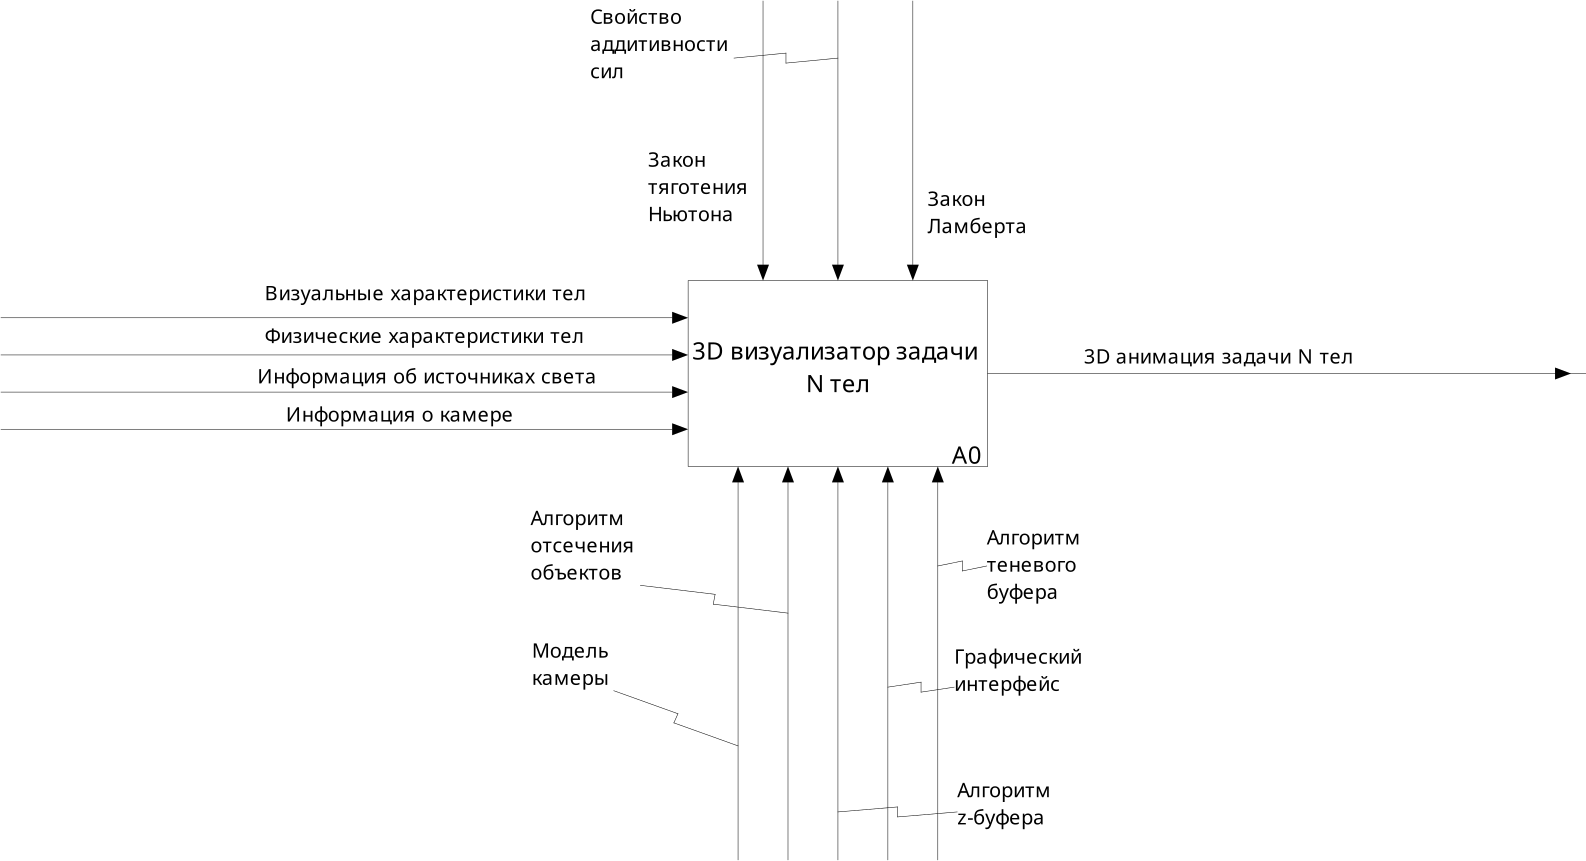
\includegraphics[width=0.9\textwidth]{ramus/01_A0}
	\caption{"Контекстная диаграмма верхнего уровня"}
	\label{fig:A0}
\end{figure}

\begin{figure}[H]
	\centering
	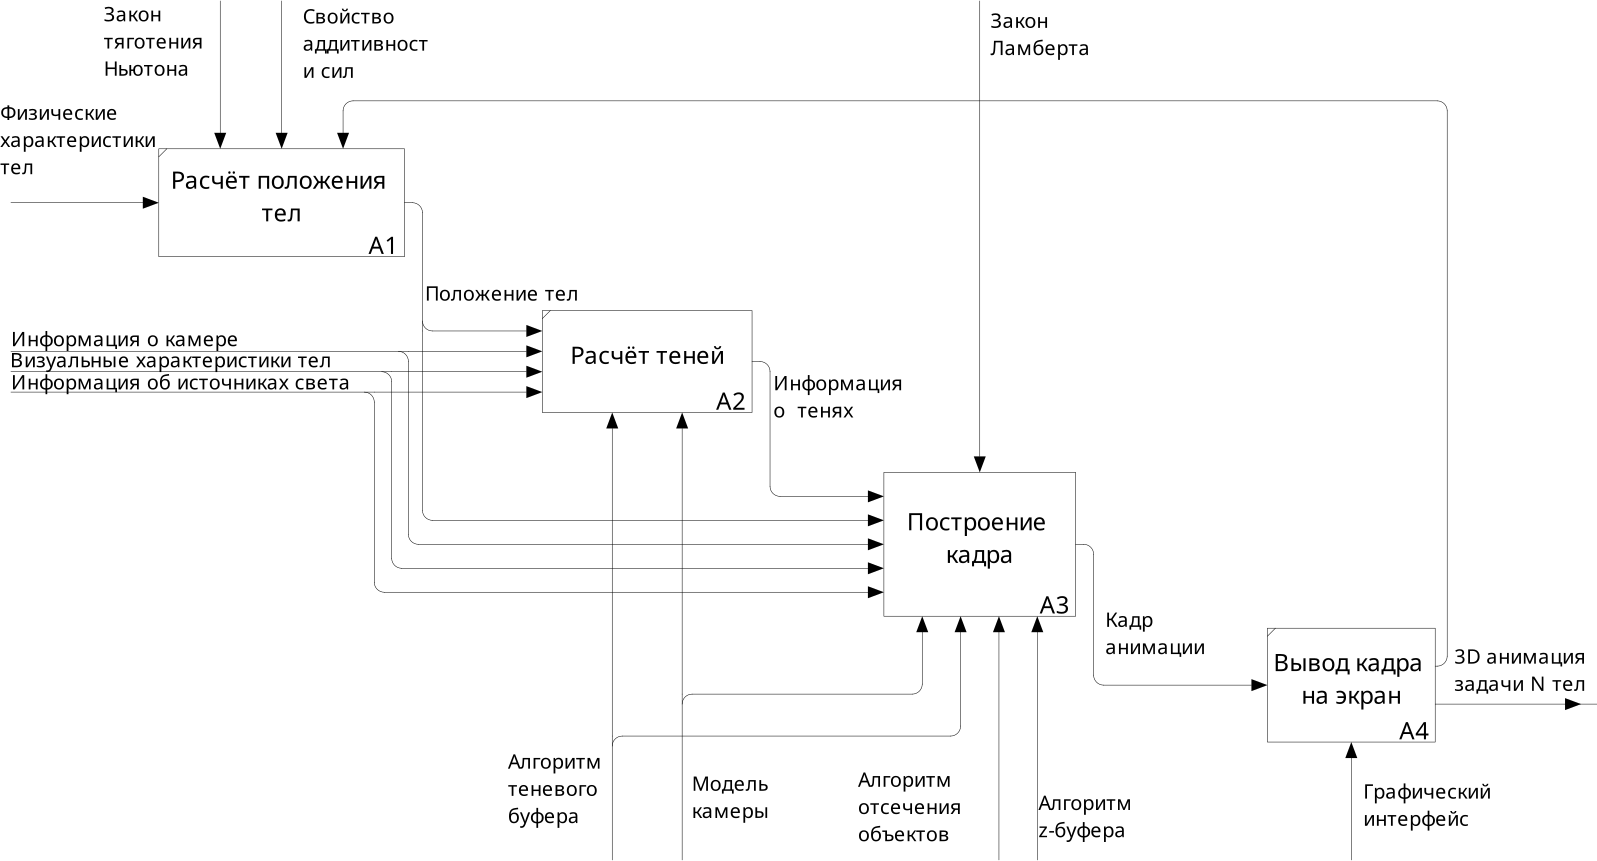
\includegraphics[width=0.9\textwidth]{ramus/02_A0}
	\caption{"Основной цикл ПО"}
	\label{fig:A1}
\end{figure}

\begin{figure}[H]
	\centering
	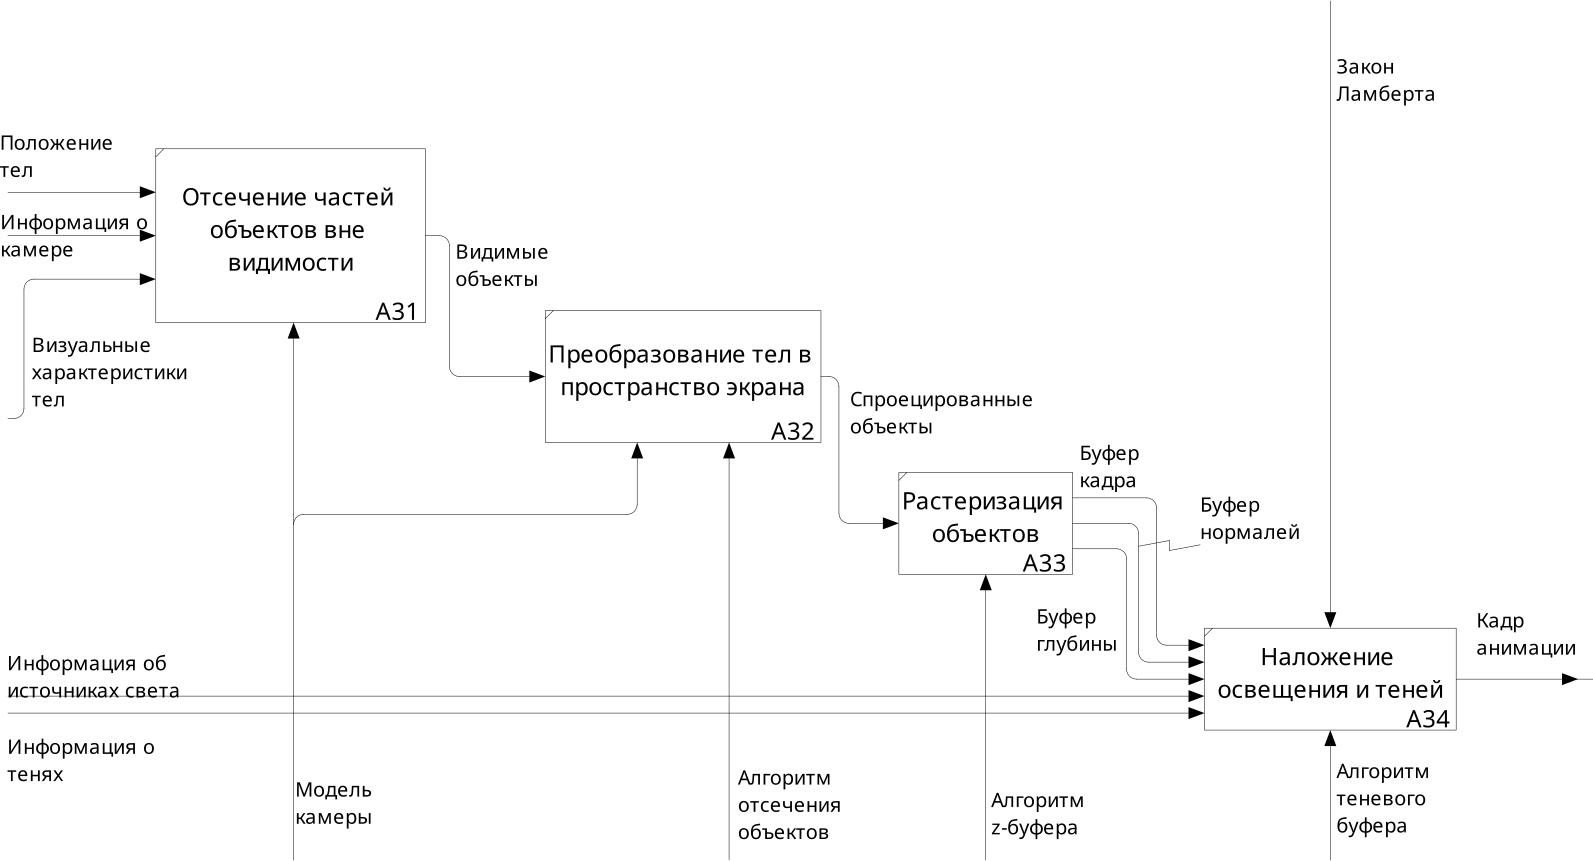
\includegraphics[width=0.9\textwidth]{ramus/03_A3}
	\caption{"Построение кадра"}
	\label{fig:A3}
\end{figure}

\section{Модель камеры}

Камера задаётся своим положением, направлением взгляда и направлением вверх и пирамидой видимости. Вектор в сторону получается векторным произведением вектора взгляда на вектор вверх. В пространстве камеры направление взгляда совпадает с положительным направлением оси z, а направление вверх -- с положительным направлением оси y.


Пирамида видимости -- усечённая 4-х гранная пирамида, уходящая в бесконечность, основание которой параллельно XoY. Основание пирамиды задаётся 3-мя параметрами:

\begin{itemize}
	\item $d$ -- расстояние от положения камеры до основания;
	\item $rx$ -- ширина основания;
	\item $ry$ -- высота основания.
\end{itemize}

Пирамида видимости в пространстве камеры продемонстрирована на рисунке \ref{fig:camera}.

\begin{figure}[H]
	\centering
	\includegraphics[width=0.5\textwidth]{camera}
	\caption{"Пирамида видимости камеры"}
	\label{fig:camera}
\end{figure}

Перспективная проекция по пирамиде видимости рассчитывается по формуле \ref{eq:perspective} \cite{projection}.

\begin{equation}
	\label{eq:perspective}
	\begin{pmatrix}
		x_p \\
		y_p \\
		z_p \\
		w_p \\
	\end{pmatrix} = 
	\begin{pmatrix}
		\frac{d}{rx}  & 0 & 0 & 0 \\
		0 & \frac{d}{ry} & 0 & 0 \\
		0 & 0 & 1 & 2d \\
		0 & 0 & 1 & 0 \\
	\end{pmatrix}
	\begin{pmatrix}
		x \\
		y \\
		z \\
		w \\
	\end{pmatrix}
\end{equation}

\section{title}

\section*{Вывод}

\clearpage
